\hypertarget{algorytm_8cpp}{\section{algorytm.\-cpp File Reference}
\label{algorytm_8cpp}\index{algorytm.\-cpp@{algorytm.\-cpp}}
}


Plik z definicjami metod dla klasy algorytm.  


{\ttfamily \#include $<$iostream$>$}\\*
{\ttfamily \#include $<$ctime$>$}\\*
{\ttfamily \#include $<$sys/time.\-h$>$}\\*
{\ttfamily \#include $<$cstdlib$>$}\\*
{\ttfamily \#include $<$cmath$>$}\\*
{\ttfamily \#include $<$fstream$>$}\\*
{\ttfamily \#include \char`\"{}algorytm.\-h\char`\"{}}\\*
{\ttfamily \#include \char`\"{}stos.\-h\char`\"{}}\\*
{\ttfamily \#include \char`\"{}kolejka.\-h\char`\"{}}\\*
Include dependency graph for algorytm.\-cpp\-:
\nopagebreak
\begin{figure}[H]
\begin{center}
\leavevmode
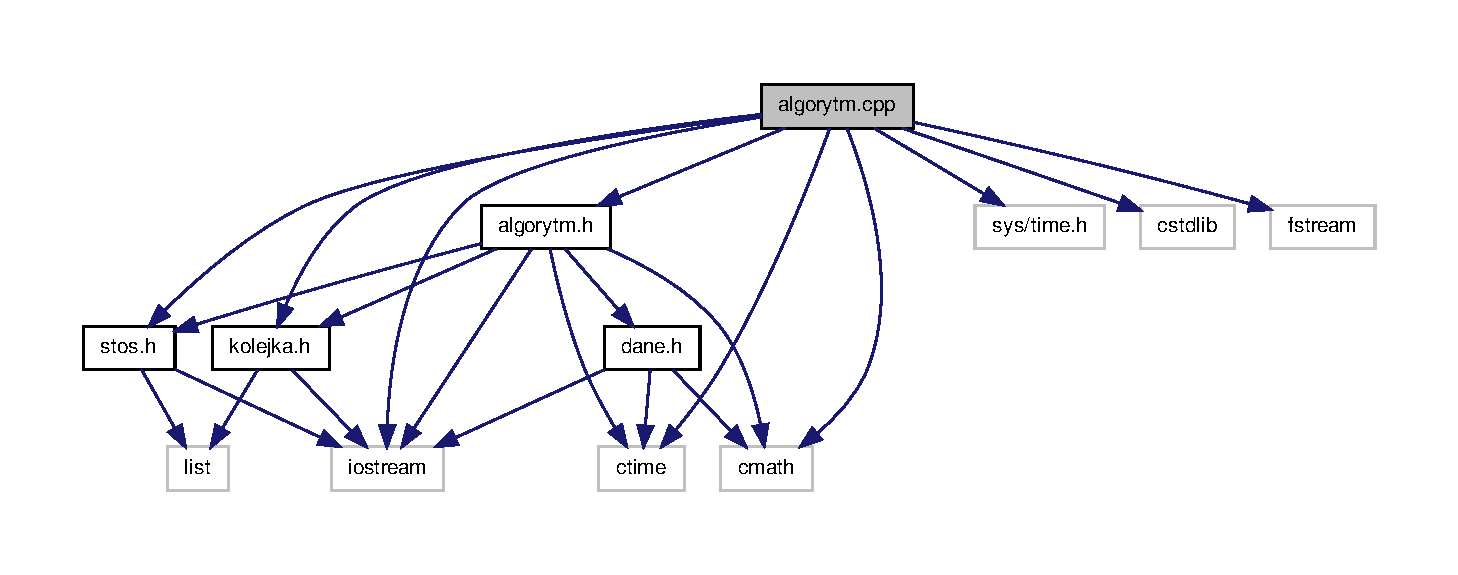
\includegraphics[width=350pt]{algorytm_8cpp__incl}
\end{center}
\end{figure}


\subsection{Detailed Description}
Plik zawiera definicje metod klasy algorytm oraz przeciazenie operatora przypisania. Zdefiniowane sa tutaj metody odpowiadajace za wczytanie pliku z danymi oraz pliku z danymi sprawdzajacymi. Ponadto zdefiniowana sa metody pobrania czasu, wykonania obliczen algorytmu, sprawdzajaca poprawnosc obliczen oraz test algorytmu. w tym miejsu również znajduja sie definicje operacji odwracania elementow tablicy, zamiany danych elementow, dodanie elementu do tablicy, dodanie dwoch tablic. Zdefiniowane sa tez pliki testowe dla operacji wczytywania danych do struktur danych min kolejki i stosu. 

Definition in file \hyperlink{algorytm_8cpp_source}{algorytm.\-cpp}.

